\newpage
\subsection{High Order DPA attacks}
\label{High_Order_DPA_attacks}


See \cite{phd-Giraud-2007}, his PhD study in detail this attack on AES, 
and see also the original article \cite{fse-2003-akkar} and \cite{ches-2001-akkar}.

We saw that testing hypothesis about a manipulated variable depending on a part of
the key, part small enough so that a brute force search could be 
undertaken, could lead to reveal the used secret key.

We saw afterwards, that this kind of threat can be prevented, simply by breaking 
the link between the manipulated value and the power consumption: this means
practically that no attacker shall be able to anticipated any sensitive manipulated 
value by technique such as masking.

In fact this kind of countermeasure can be bypassed, by another class of side 
channel attack generalization of the DPA seen previously. Instead of doing hypothesis
on one manipulated variable, those Hight Order DPA attacks do hypothesis one multiple 
intermediate value.

      \begin{figure}[!h]
        \centering
        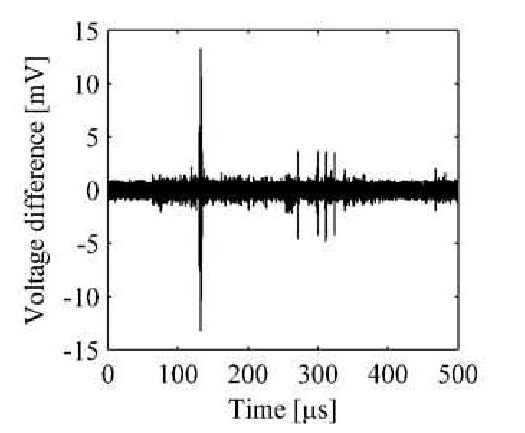
\includegraphics[width=10cm,height=3cm]{images/dpa_result.png}
        \caption{Successful DPA attack}
      \end{figure}	
      
More than the number of sub key hypothesis -which is squared for HODPA square- the 
main difference between DPA and -true- HODPA is that DPA attack 
target one variable manipulated in moment in time, $\tau$ whereas HODPA 
target multiple variable manipulate at moment in time $\tau_1$, $\tau_2$, ...

      \begin{figure}[!h]
        \centering
		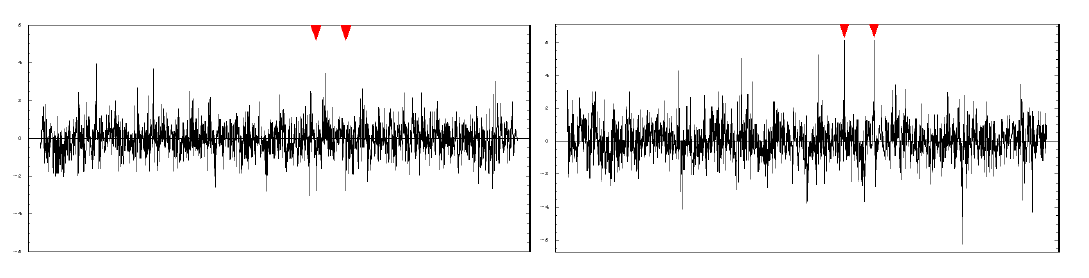
\includegraphics[width=14cm,height=3cm]{images/hodpa_result.png}
		\caption{Unsuccessful \textit{vs} successful HODPA attack}
      \end{figure}	

\subsubsection{A particular case: The superposition attack}
\label{The_superposition_attack}

The superposition attack proposed by M-L.Akkar and L.Goubin against their own implementation 
' the Transforming masking method', see \ref{The_Transforming_Masking_Method}.
This is a second order DPA attack in theory because the selection function used is function of two distinct 
sub-keys. But in practice, it is nearly as simple as an usual DPA attack. '\#1.333 HODPA'
\vspace{3mm}
 
The idea is as following: in a second order DPA attack, the most
difficult thing is to localize the time when the precise needed values are manipulated,
but on the contrary, localizing a whole DES round is often quite easy.
So instead of correlating precise parts of the consumption traces, the attacker
will just correlate the whole trace of the first and the last round.
\vspace{3mm}

The main idea is to perform a front attack with a plain-text $M$, making an hypothesis
on a part of $K_1$, in the same time to perform a back-end attack with a cypher text $C$,
making another hypothesis on a part of $K_16$.
For one S-Box there will have 4096 possibilities for a sub-key hypothesis.\\
As we can see, by example with picture \textit{26} , every output of SM-Box are masked 
with a value depending on the main mask,
the thing that allow an attack to be possible is the fact that the value
$P^{-1}( R1_{0-31}\oplus R1_{32-63})$ is always the same.

Then  we have:
\begin{center}
$T =    S(EP(IP^{-1}(C)_{32-63}) \oplus K_{16}) \oplus P^{-1}(IP(R)_{32-63} \oplus IP(R)_{0-31})) $

$\oplus S(E(IP(M)_{32-63}) \oplus K_1) \oplus P^{-1}(IP(R)_{32-63} \oplus IP(R)_{0-31})))$\\  
\end{center}
\begin{center}
$T = S(E(IP^{-1}(C)_{32-63}) \oplus K_{16}) \oplus S(E(IP(M)_{32-63}) \oplus K_1)$
\end{center}

Key idea : that the value $T$ does not depend on the random masking value.

On the next page is explained the different step of the algorithm, one can note that 
the presented version, taken from \cite{fse-2003-akkar}, is a mono-bit DPA attack and 
that T.Messerge's multi-bit attack, would also work just like a CPA attack.


			\begin{algorithm}[h]
				\KwIn{Curves resulting of the addition of traces from round 1 and 16 }
				$y \leftarrow 1$	\;	
					\For{$i=0 \mbox{ } j<64 \mbox{ }i++ $ }{			 
						 \For{$j=0 \mbox{ } j<64 \mbox{ }j++ $ }{			 
							 \For{ All the Curves }{			 
					Separate the curves in two packets depending on one bit of the part of $T$ which is
					corresponding to the attacked S-box and assuming that the part of $K_1$ and $K_{16}$
					corresponding to the attacked S-box are $i$ and $j$.\\
					Average and subtract the separated curves.
							} 
						} 	
					}
					Choose the value of $i$ and $j$ where the greatest peak appears.\\
					Check the coherency the $i$ and $j$ has to be compatible. 	\;							 
				\Return{$ i,j $}\;
				\caption{Superposition Attack on S-boxes}
			\end{algorithm}

Note that this algorithm requires as an input to sum two round of a DES, if there is 
a problem of alignment this will dangerously compromise the attack.


\newpage
\subsubsection{General HODPA}
\label{eneral_HODPA}

	
In classical DPA attack once that the trace have been processed to remove noise, aligned and so on
it sure that if an attack was launched on those traces then peaks would occurred exactly when the 
targeted variable is manipulated.  This is assuming few hypothesis:
\begin{itemize}
	\item power consumption was measured while the targeted variable was manipulated
	\item a relevant power model is available and compatible with the countermeasure.
\end{itemize}

In HODPA as multiple manipulate variable are targeted, and as those variables
are manipulated at different moment in time, let's say $\tau_1$ and $\tau_2$,  
it wouldn't make any sense to launch this attack on recorded trace, 
the trace to be process align and then separate in packet are in 
fact traces that have not been recorded.
\vspace{3mm}


$\mathcal{T}_i(t)$, attacked traces, for HODPA targeting two variables,
in function of $\mathcal{C}_i(t)$ the recorded trace:

\begin{center}
$ \mathcal{T}_i(t) = \mathcal{C}_i(t)  -  \mathcal{C}_i(t + \tau_2 -\tau_1) $
\end{center}

This way for $t = \tau_1$ the fist contribution of the attacked curve 
$\mathcal{C}_i(t) $ will give pike relative to the manipulation of the first variable while at the 
the second contribution of the attacked curve $ \mathcal{C}_i(t + \tau_2 -\tau_1)$ 
will give pike relative to the manipulation of the second variable.
Morality: with such a trace $\mathcal{T}_i(t)$, peak will pop up at $t =\tau_1$
revealing that the the two targeted variable are manipulated at $\tau_1$ and $\tau_2$, .
Note that on a natural case, $\tau_2 -\tau_1$ is not known , moreover  $\tau_2$  and $\tau_1$,
then all the possibility would have to be tested .... Huge increase of the complexity.



